% Chapter 3

\chapter{TCN in common sequence dataset} % Main chapter title

\label{Chapter3} % For referencing the chapter elsewhere, use \ref{Chapter1} 

%----------------------------------------------------------------------------------------

As we addressed in \ref{Chapter1}, there are many kinds of data have the feature successive in time in common, and scholars from different research area contributed multiple views, methods, and tools to do modeling; so it is quite massive for us to have a concise plan for further work if we go through papers one by one. Instead, we will use TCN and other mainstream models(introduced in \ref{Chapter2}) and apply them to different data sets. And we also want to find an ideal data set for further experiments and implement our own research framework through such a simple reproducing and comparison. 

\section{Data Describution}

\subsection{Sequential MNIST, Digit classification}
The MNIST handwritten digit data set is widely used as a benchmark dataset for regular supervised learning. While a 2-D image of a digit does not look complex to a human being, it is a highly inefficient way for a computer to represent a handwritten digit; only a fraction of the pixels are used. Furthermore, there is a lot of regularity in digits that are not exploited by a 2-D image encoding; all digits consist of continuous line segments, produced by pen strokes. That means the model does not get to see/generate the whole image at once, but only one pixel at a time sequentially. 
\begin{figure}[H]
    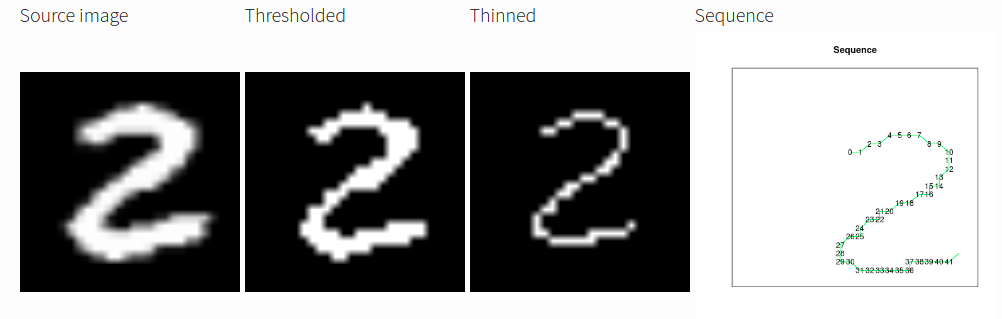
\includegraphics[width=\textwidth]{../Figures/seqMNIST.png}
    \caption{Illustrate of Sequential MNIST}
    \label{fig:MNIST}
\end{figure}
\subsection{JSB Chorales, Music}
The JSB chorales are the most commonly-used benchmark for measuring the performance of polyphonic music models to date. They are a set of short, four-voice pieces well-noted for their stylistic homogeneity. The chorales were originally composed by Johann Sebastian Bach in the 18th century. He wrote them by first taking pre-existing melodies from contemporary Lutheran hymns and then harmonising them to create the parts for the remaining three voices. The version of the dataset used here consists of 382 such chorales, with a train/validation/test split of 229, 76 and 77 samples respectively. Each input is a sequence of elements. Each element is an 88-bit binary code that corresponds to the 88 keys on a piano, with 1 indicating a key that is pressed at a given time.

\subsection{PennTreebank, LM}
The Penn Treebank, in its eight years of operation (1989-1996), produced approximately 7 million words of part-of-speech tagged text, 3 million words of skeletally parsed text, over 2 million words of text parsed for predicate-argument structure, and 1.6 million words of transcribed spoken text annotated for speech disfluencies. The material annotated includes such wide-ranging genres as IBM computer manuals, nursing notes, Wall Street Journal articles, and transcribed telephone conversations.

\section{Numeric results}
\begin{table}[H]
\centering
\caption{Model Performance Comparasion on synthetic stress tests}
\begin{tabular}{l r r r r}
\toprule
\textbf{Task} & \multicolumn{4}{c}{Models}\\
& TCN&GRU&RNN&LSTM\\
\midrule
Sequential MNIST & 87.2&96.2&21.5&99.0\\
JSB Chorales & 8.45&8.43&8.91&8.10 \\
PennTreebank& 78.93&92.48&114.50&88.68\\
\bottomrule
\end{tabular}
\label{tab:ch3-tcn}
\end{table}

\section{Limitation}
This section reproduced three kinds of sequence modeling tasks in Shaojie Bai(2018): digit classification, polyphonic music, and word-level language modeling. And TCN model showed power over other models. But one thing is that these datasets are offered by university labs and were elaborative pre-preprocessed already and might make significance in new model checking than reality applications. And although music and text could indeed be regarded as sequence tasks, we want to find whether TCN could deal with more common and pure time-series featured datasets, like stock price, traffic load, or energy supply load. 

So that we want to apply TCN into more reality tasks, at first, we use TCN to model the stock index, Dow Jones Industrial Average. Although we could fit a model with 90\% accuracy based on historical data, we do not have high confidence it could perform well in the future or other symbols in the finance market since there is much abrupt noise during everyday trading, we hardly could accuracy label where is an "anomaly period" in time. Therefore, in the next experiment, we will use grid load data to do further work.
